\section{Experimental Results}\label{sec:results}

In \S\ref{sec:superswarm}, we evaluate \olmix---using \fullmixreuse and \partialmixreuse, with recomputation done via \base---in an LM development setting where the domain set evolves through several updates. In \S\ref{sec:validation}, we empirically validate our results from \S\ref{sec:analysis}, confirming that our theoretical analysis accurately characterizes mixture reuse performance in practice.


\subsection{Real-World LM Development Scenario}\label{sec:superswarm}

We evaluate \fullmixreuse and \partialmixreuse across a sequence of five domain updates mirroring real-world LM development. Our results show that these methods maintain strong performance while substantially reducing computational costs compared to full recomputation.

\subsubsection{Setup}

See Appendix~\ref{supp:exp_details} for full experiment details on evaluation tasks and the $1$B target models we train.

\textbf{Domain Updates} We simulate a real-world LM development workflow with an initial web corpus that undergoes 5 updates (Table~\ref{tab:domain-updates-full}). 
The final domain set contains 64 domains (token counts in Table~\ref{tab:domain_sizes}).

\begin{table}[!h]
\centering
\caption{Datasets used for simulated domain updates.}
\small
\begin{tabular}{l p{0.6\linewidth} r}
\toprule
\textbf{Operation} & \textbf{Dataset(s)} & \textbf{$\Delta m$} \\
\midrule
Initial &
DCLM~\citep{dclm} partitioned into topical domains using WebOrganizer~\citep{wettig2025organizewebconstructingdomains}) &
24 \\
\midrule
\Add &
Stack-Edu~\citep{allal2025smollm2smolgoesbig}, partitioned by programming language &
+15 \\
\Add &
ArXiv~\citep{azerbayev2023llemma}, FineMath~3+~\citep{allal2025smollm2smolgoesbig}, olmOCR Science PDFs~\citep{olmo2025olmo3}, Dolma 1 Wikipedia~\citep{soldaini2024dolma}, AlgebraicStack~\citep{azerbayev2023llemma}, pes2o~\citep{peS2o} &
+6 \\
\Revise &
olmOCR Science PDFs~\citep{olmo2025olmo3} (reformatted tables and references) &
0 \\
\Remove &
AlgebraicStack~\citep{azerbayev2023llemma} &
$-1$ \\
\Partition &
olmOCR Science PDFs~\citep{olmo2025olmo3}, partitioned into topical domains using WebOrganizer~\citep{wettig2025organizewebconstructingdomains} &
+20 \\
\bottomrule
\end{tabular}
\label{tab:domain-updates-full}
\end{table}

\textbf{Methods compared.} We consider:
\begin{itemize}[itemsep=0pt,topsep=0pt,leftmargin=12pt]
    \item Natural: mix proportional to domain sizes.
    \item Full recomputation: apply \base after each update (high performance, high cost).
    \item Swarm reuse: reuse all accumulated proxy runs that can represented on $\D'$ and apply \base on the combined swarm (see Algorithm~\ref{alg:swarm_reuse_method}). 
    \item \fullmixreuse (our method): reuse ratios for unaffected domains, recompute affected ones. 
    \item \partialmixreuse (our method): reuse ratios within DCLM topics and within Stack-Edu languages while recomputing at the source level; recompute DCLM:software development when adding Stack-Edu due to high coupling (see \S~\ref{sec:validation_results} for justification).
\end{itemize}




\textbf{Experimental protocol.} 
For full recomputation, we use swarm size $K \approx c(m + 1)$ and vary $c \in \{1, 2, 3\}$ to showcase different compute regimes. For swarm reuse and mixture reuse, we set swarm sizes to roughly match that of full recomputation with $c=1$.
We report results over $3$ random seeds of swarms with $k=4$, $R=1$T. Full details are in Appendix~\ref{supp:imp_details}.


\begin{figure}[H]
    \centering
    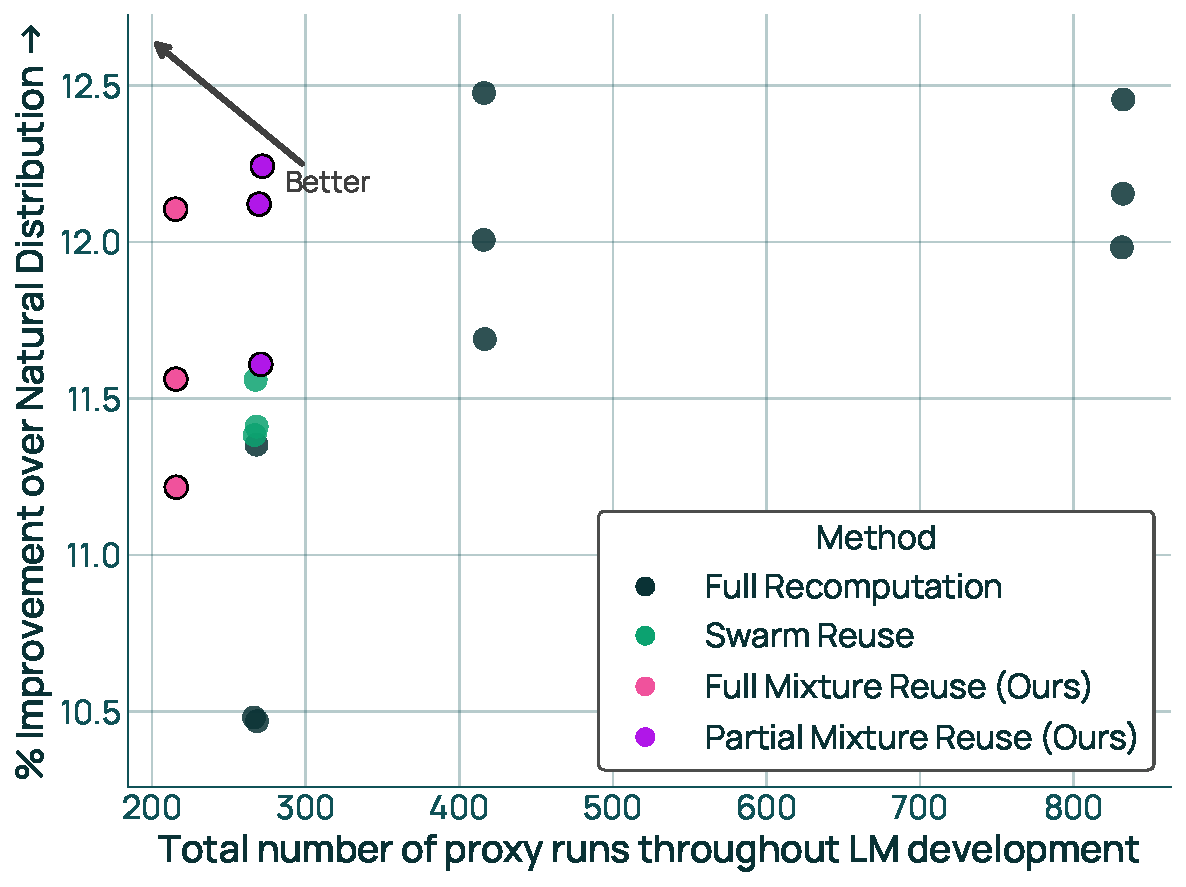
\includegraphics[width=0.6\linewidth]{figs/contribution_2/superswarm_1T.pdf}
    \caption{Performance improvement versus cost of mixing under evolving domains. \fullmixreuse and \partialmixreuse achieve $>95\%$ of the improvement of full recomputation while using at least $67\%$ fewer proxy runs.}
    \label{fig:main_results}
\end{figure}


\subsubsection{Results}\label{sec:results_1}

See Appendix~\ref{sec:additional_exp_results} for additional results on: 1) $R=6$T, 2) smaller proxy run budgets, and 3) individual domain update operators.

\textbf{\fullmixreuse roughly matches full recomputation at substantially lower cost.} Figure~\ref{fig:main_results} shows relative improvement in downstream performance (average BPB) over the natural distribution versus the total number of proxy runs across all 5 updates. \fullmixreuse achieves 95\% of full recomputation's ($c\texttt{=}3$) performance improvement (+11.6\% versus +12.2\%) while using 74\% fewer total proxy runs (216 versus 832). 

\textbf{\partialmixreuse closes the remaining gap between \fullmixreuse and full recomputation.}
By selectively recomputing some unaffected domains, \partialmixreuse achieves 98\% of full recomputation's performance (+12.0\%) with 272 total runs---still 67\% fewer than full recomputation. 


\textbf{Mixture reuse outperforms swarm reuse.}
Swarm reuse achieves +11.4\% with 268 runs, underperforming \fullmixreuse (+11.6\% with 216 runs) despite using more runs. This is likely because (1) representing old swarms on updated domain sets over-explores biased subspaces, and (2) swarms cannot be reused when domains are removed or revised.


\textbf{At matched proxy run budgets, mixture reuse outperforms alternatives.} 
At a budget of 216-272 proxy runs, \fullmixreuse and \partialmixreuse achieve +11.6\% and +12.0\% improvement over the natural distribution, respectively. At this same budget, swarm reuse achieves +11.4\% and full recomputation achieves +10.8\% ($c=1$). 



\textbf{Our best mixture is 3.05× more data-efficient than the natural distribution.}
Beyond final performance, we measure data efficiency: how many training steps does our best learned mixture need to match the natural distribution's final performance? Figure~\ref{fig:checkpoints} shows that \partialmixreuse reaches the natural distribution's final BPB in approximately 20,000 steps versus 61,000 steps---a 3.05× speedup.


\begin{figure}
    \centering
    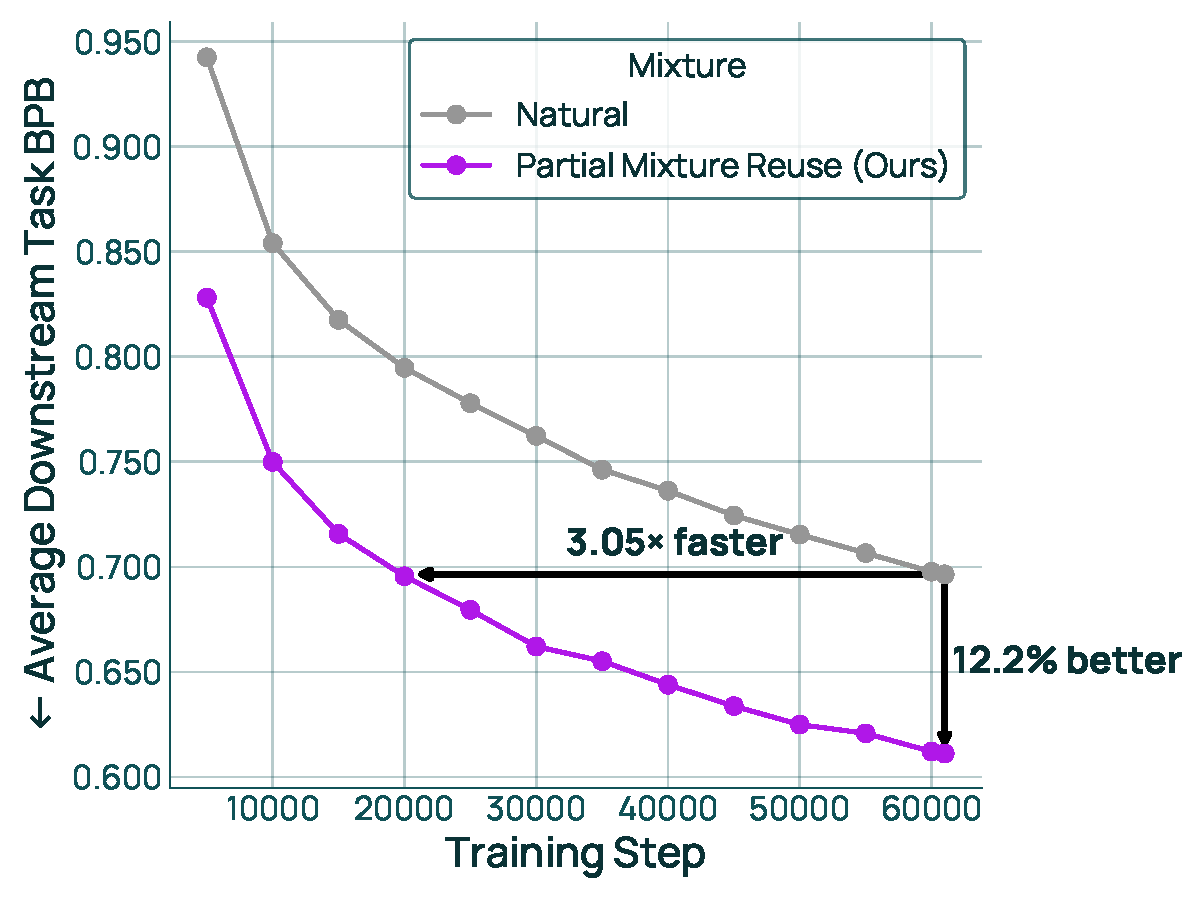
\includegraphics[width=0.6\linewidth]{figs/contribution_2/checkpoint_comparison.pdf}
    \caption{Downstream performance across training for \partialmixreuse (best seed) versus the natural distribution. \partialmixreuse reaches the natural distribution's final performance in 3.05$\times$ fewer steps.}
    \label{fig:checkpoints}
\end{figure}

\textbf{Qualitative analysis of learned mixtures.}
Figure~\ref{fig:superswarm_proposed_mixes} shows the final proposed mixes over a subset of domains (full mix in Table~\ref{tab:full_domain_mixtures}). \partialmixreuse is more similar to full recomputation (total variation distance of 0.067) than to the natural distribution (distance of 0.127), aligning with our downstream performance findings.



\begin{figure}
    \centering
    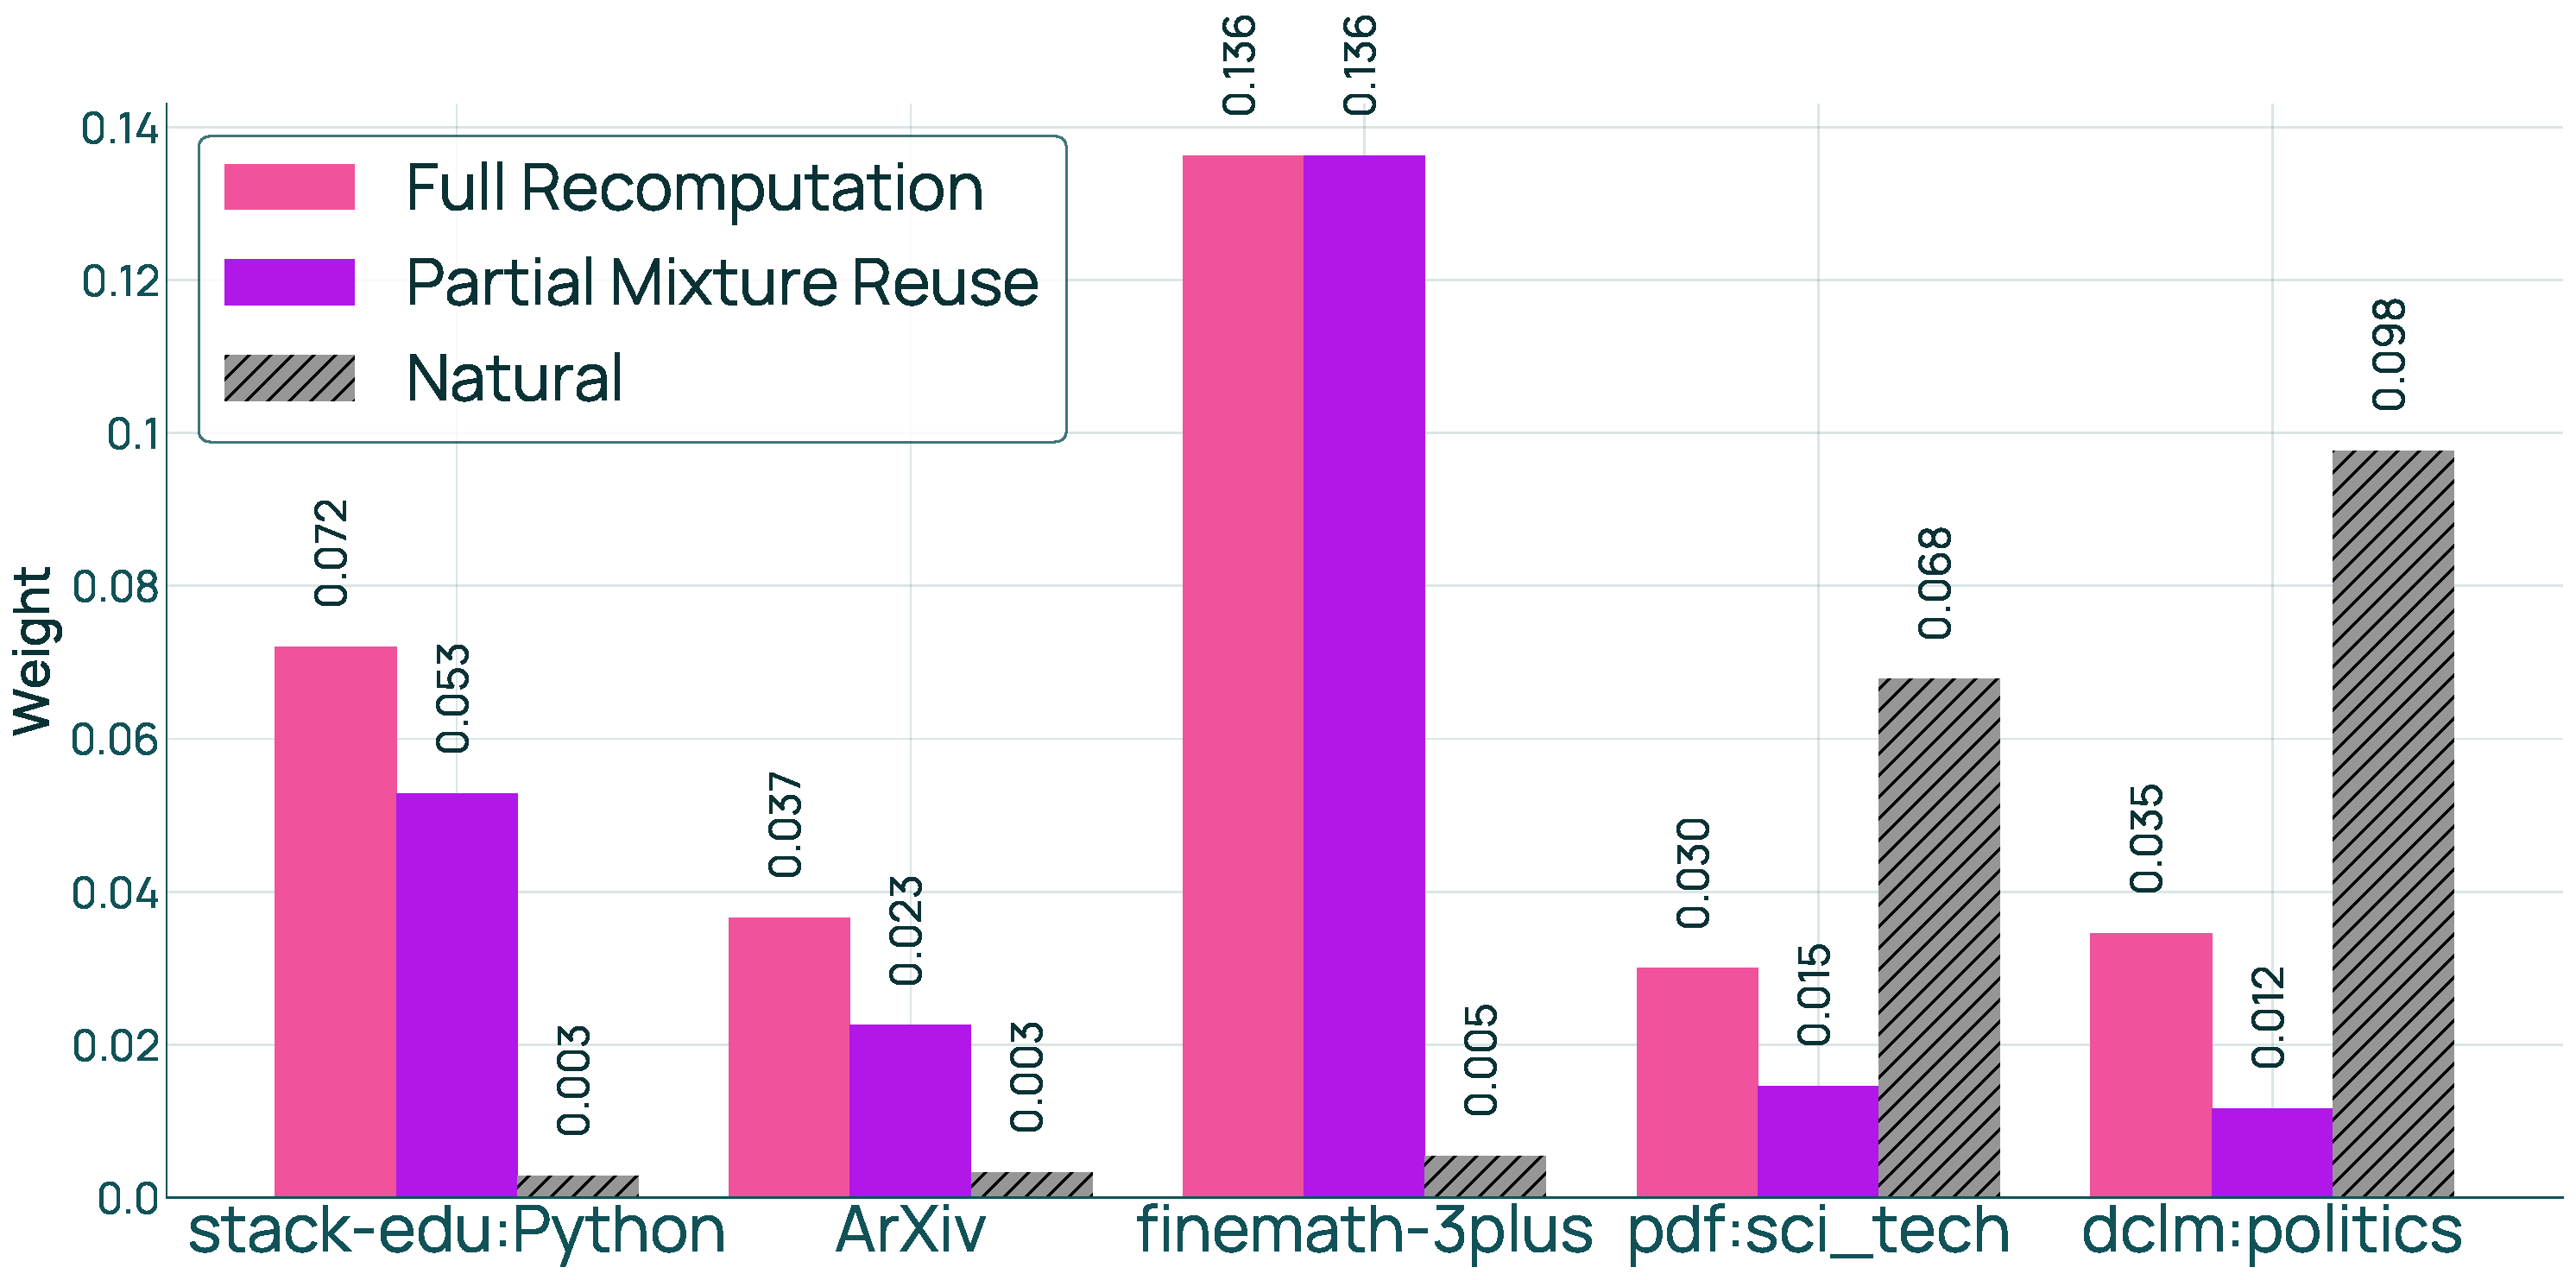
\includegraphics[width=0.8\linewidth]{figs/contribution_2/superswarm_mix_comparison_top5.pdf}
    \caption{Proposed mixes for different mixing strategies. The mixes produced by full recomputation and \partialmixreuse are more similar to each other than they are to the natural distribution, confirming the performance results in Figure~\ref{fig:main_results}. Domains shown have the greatest difference in weights between full recomputation and natural.}
    \label{fig:superswarm_proposed_mixes}
\end{figure}




\subsection{Empirical Validation of Theorems~\ref{thm:general_gap} and~\ref{thm:add_domains}}\label{sec:validation}

We empirically measure the terms in Theorems~\ref{thm:general_gap} and~\ref{thm:add_domains} to assess whether they track the performance of mixture reuse.

\subsubsection{Setup}

We consider two examples of an \Add update:
\begin{itemize}
    \item $\D_1=$DCLM~\citep{dclm} partitioned into 24 topic-based domains using WebOrganizer~\citep{wettig2025organizewebconstructingdomains}, $\D_2'$ = Stack-Edu~\citep{allal2025smollm2smolgoesbig} partitioned into $15$ programming languages.
    \item $\D_1=$DCLM partitioned into 24 topic-based domains using WebOrganizer, $\D_2'$ = olmOCR Science PDFs~\citep{olmo2025olmo3} partitioned into $21$ topic-based domains using WebOrganizer. 
\end{itemize}

\subsubsection{Results}\label{sec:validation_results}


\textbf{Performance is correlated with the reuse gap.} 
Mixture reuse yields $q^\star(\tilde{p}_{\Dfix})$ from Algorithm~\ref{alg:conditional_mixing_method} given reused ratios $\tilde{p}_{\Dfix}$. Full recomputation yields $q^\star$ from directly solving~\eqref{eq:mixing_problem} for the optimal mix on $\D'$.
Theorem~\ref{thm:general_gap} shows that the performance gap of mixture reuse, $F(q^\star(\tilde{p}_{\Dfix})) - F(q^\star)$, where $F$ is the average downstream task BPB, is bounded in terms of the reuse gap, $\|\tilde{p}_{\Dfix} - q_{\Dfix}^\star \|$, where $q_{\Dfix}^\star$ is $q^\star$ normalized over $\Dfix$. We validate that the reuse gap predicts the performance gap.


To do this, we construct different values of $\tilde{p}_{\Dfix}$ with varying reuse gaps and measure the resulting performance gaps.
We first approximate $q_{\Dfix}^\star$ (and $F(q^\star)$) by running full recomputation on $\D'$ using \base and normalizing the resulting mix over $\Dfix$. 
We then construct two $\tilde{p}_{\Dfix}$:
\begin{itemize}
    \item Weak mix: to construct a $\tilde{p}_{\Dfix}$ far from $q^\star_{\Dfix}$, we run \base on $\D'$ with a modified objective that maximizes BPB and then normalize the resulting mix over $\Dfix$.
    \item Intermediate mix: we average the weak mix with $q^\star_{\Dfix}$.
\end{itemize}

Figure~\ref{fig:theorem1_validation} confirms the findings of Theorem~\ref{thm:general_gap}: as the reuse gap increases, the performance gap also increases across both settings.


\begin{figure}
    \centering
    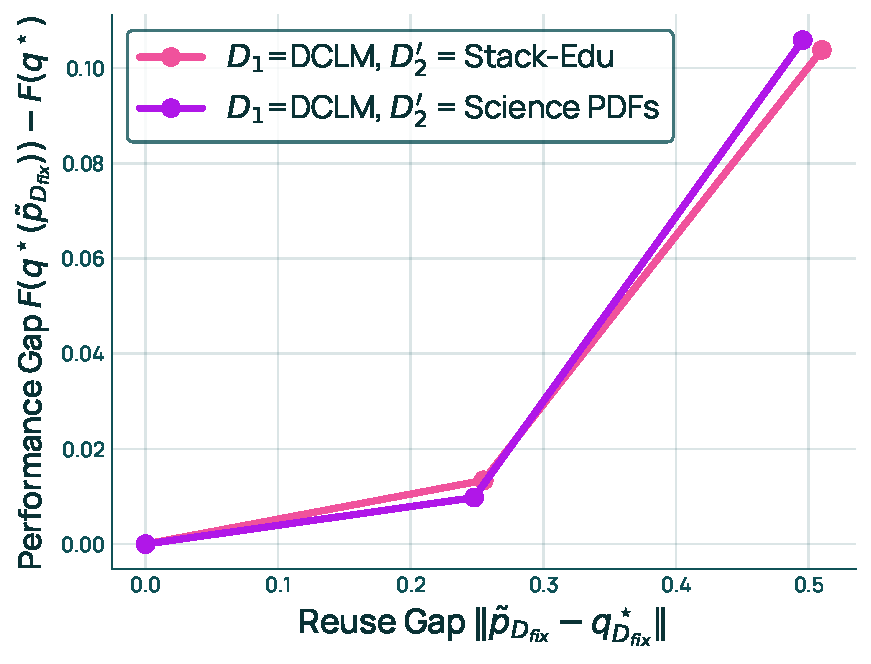
\includegraphics[width=0.4\linewidth]{figs/contribution_2/theorem1_validation.pdf}
    \caption{Performance vs Reuse Gap. The optimality of $\tilde{p}_{\Dfix}$ after the domain update is correlated with the success of mixture reuse.}
    \label{fig:theorem1_validation}
\end{figure}

\textbf{The reuse gap is controlled by how much the domain update shifts the optimal mixture.}
When adding domains, Theorem~\ref{thm:add_domains} shows that the reuse gap (and consequently the performance gap) depends on how much total weight shifts to the affected domains. Specifically, the reuse gap depends on $1 - \rho^\star$, where $\rho^\star$ is the total weight on the reused domains $\D_1$ in the optimal mix $q^\star$.
We validate that $1 - \rho^\star$ predicts both the reuse gap and performance gap.

To do this, we construct settings with different $\rho^\star$ by varying the repetition constraint. A tight constraint (small $k$ or large $R$ in~\eqref{eq:mixing_problem}) forces the mix to stay close to the natural distribution, yielding $\rho^\star \approx 1$ when $\D_1$ is much larger than the added domains. A relaxed constraint allows more weight to shift to new domains, potentially yielding smaller $\rho^\star$.
We test two settings: $R = 1$T (relaxed) and $R = 6$T (tight). For each $R$, we 1) compute $\tilde{p}_{\Dfix}$ by running \base on $\D$; 2) apply \fullmixreuse on $\D'$ using $\tilde{p}_{\Dfix}$; and 3) use full recomputation (run \base on $\D'$) to get an approximate $\rho^\star$, the reuse gap, and the performance gap.


Figure~\ref{fig:theorem2_validation} shows that larger $1 - \rho^\star$ correlates with both a larger reuse gap and a larger performance gap across both settings, validating that the extent to which the domain update shifts the optimal mixture directly impacts mixture reuse performance.


\begin{figure}
    \centering
    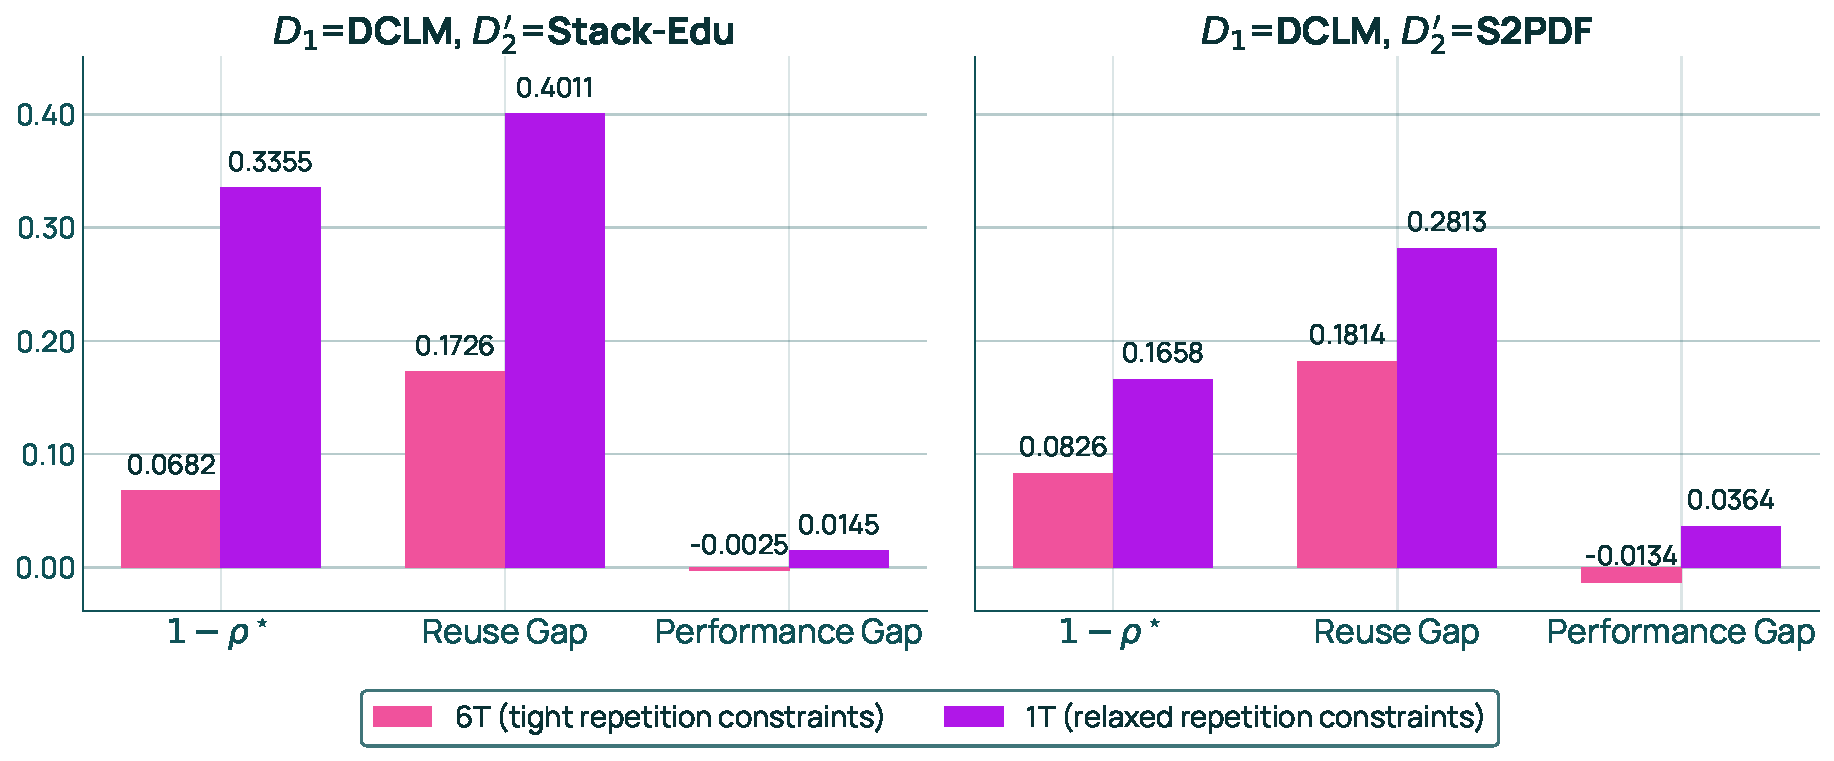
\includegraphics[width=\linewidth]{figs/contribution_2/theorem2_validation_combined.pdf}
    \caption{Performance gap vs reuse gap vs $1 - \rho^\star$ when adding Stack-Edu to DCLM (left) and olmOCR Science PDFs to DCLM (right). Varying $R$ changes $\rho^\star$, and we observe that $1 - \rho^\star$ propagates to both the reuse gap and performance gap, validating Theorem~\ref{thm:add_domains}.}
    \label{fig:theorem2_validation}
\end{figure}



\textbf{\partialmixreuse reduces coupling and improves performance.}
Theorems~\ref{thm:general_gap} and~\ref{thm:add_domains} show that the coupling term $\kappa$ controls the \emph{rate} at which changes in optimality translate to the performance gap. The coupling term is large when both reused domains $\Dfix$ and recomputed domains $\Dcomp$ impact similar downstream tasks.
We validate that reducing coupling---by adjusting $\Dfix$ vs $\Dcomp$ via \partialmixreuse---improves both the reuse gap and performance gap.


To do this, we analyze a scenario where coupling is high: adding Stack-Edu to DCLM topics when $R=1$T (from Figure~\ref{fig:theorem2_validation} left, purple). 
Figure~\ref{fig:theorem2_validation_dclm_mix} compares the reused ratios $\tilde{p}_{\Dfix}$ against the optimal ratios $q^\star_{\Dfix}$ over DCLM topics. There is a stark difference in the weight on DCLM's software development topic, suggesting high coupling between software development and Stack-Edu.
Based on this, we test whether \partialmixreuse with $\Dcomp = \text{Stack-Edu} \cup \{\text{DCLM:software\_development}\}$ reduces coupling and improves performance compared to \fullmixreuse (which uses $\Dcomp = \text{Stack-Edu}$).

\begin{figure}
    \centering
    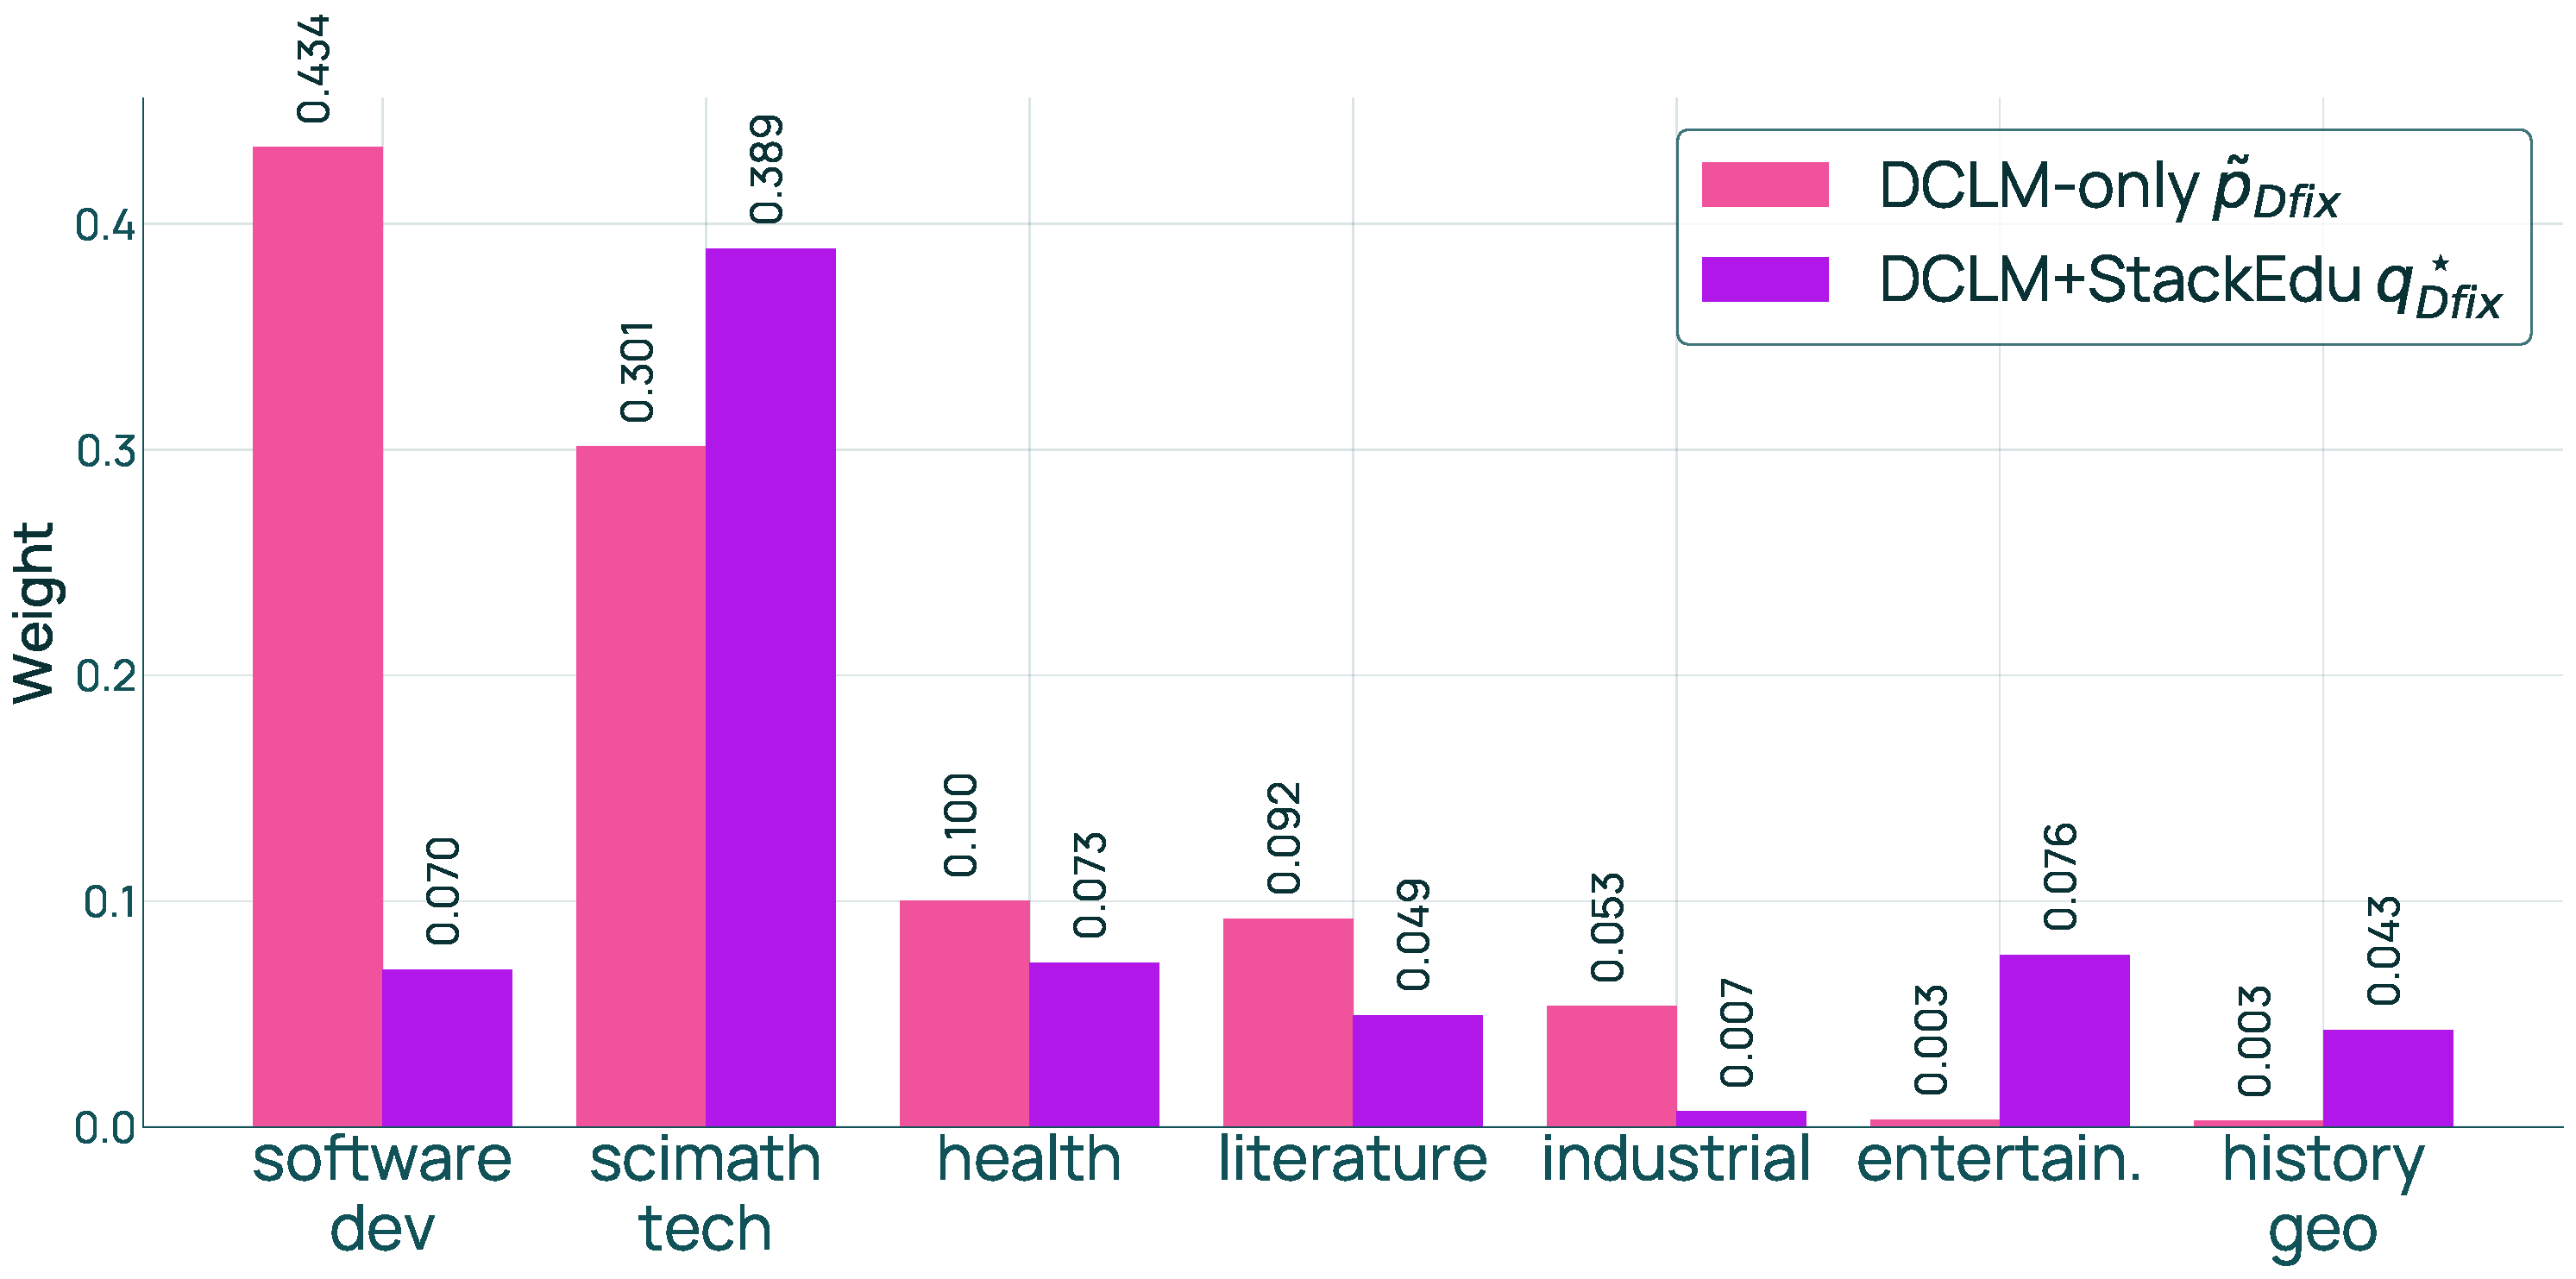
\includegraphics[width=0.6\linewidth]{figs/contribution_2/theorem2_validation_dclm_mix.pdf}
    \caption{Comparison of $\tilde{p}_{\Dfix}$ versus $q^\star_{\Dfix}$ (top-7 domains according to $\tilde{p}_{\Dfix}$) when $\D_1=$DCLM, $\D_2'$=Stack-Edu with $R=1$T. The only domain that significantly differs in mixture weight is software development, suggesting that \partialmixreuse can reduce coupling if we recompute DCLM:software\_development.}
    \label{fig:theorem2_validation_dclm_mix}
\end{figure}

Figure~\ref{fig:theorem2_validation_coupling} shows that recomputing DCLM:software\_development along with Stack-Edu reduces both the reuse gap and performance gap, despite $1 - \rho^\star$ being larger for \partialmixreuse. This breaks the pattern seen in Figure~\ref{fig:theorem2_validation}: larger $1 - \rho^\star$ no longer translates to a larger performance gap, suggesting that the reduction in the coupling term $\kappa$ dominates.
To confirm this directly, we compute $\kappa$ (see Appendix~\ref{supp:defs} for definition) for \fullmixreuse and $\kappa$ for \partialmixreuse with $\Dcomp = \text{Stack-Edu} \cup \{\text{DCLM:topic} \}$ for each DCLM topic.
Figure~\ref{fig:theorem2_validation_kappa_reduction} shows that recomputing DCLM:software\_development reduces $\kappa$ far more than recomputing any other DCLM topic, validating that \partialmixreuse reduces coupling.



\begin{figure}
    \centering
    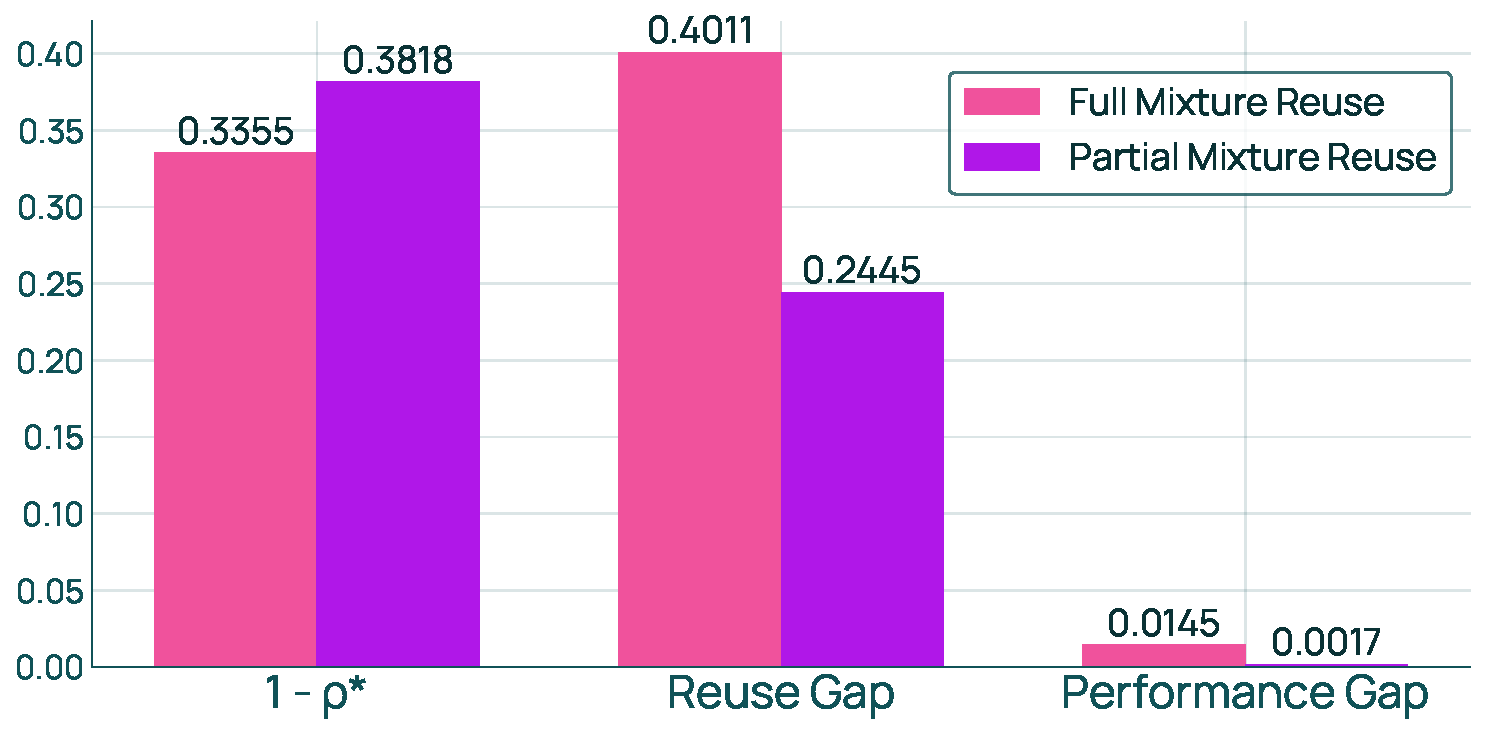
\includegraphics[width=0.6\linewidth]{figs/contribution_2/theorem2_validation_coupling.pdf}
    \caption{Performance of \partialmixreuse (recompute DCLM:software\_development) for $\D_1$=DCLM, $\D_2'$=Stack-Edu with $R=1$T. Recomputing DCLM:software development along with Stack-Edu reduces both the reuse gap and the performance gap, even though its $1 - \rho^\star$ is higher.}
    \label{fig:theorem2_validation_coupling}
\end{figure}

\begin{figure}
    \centering
    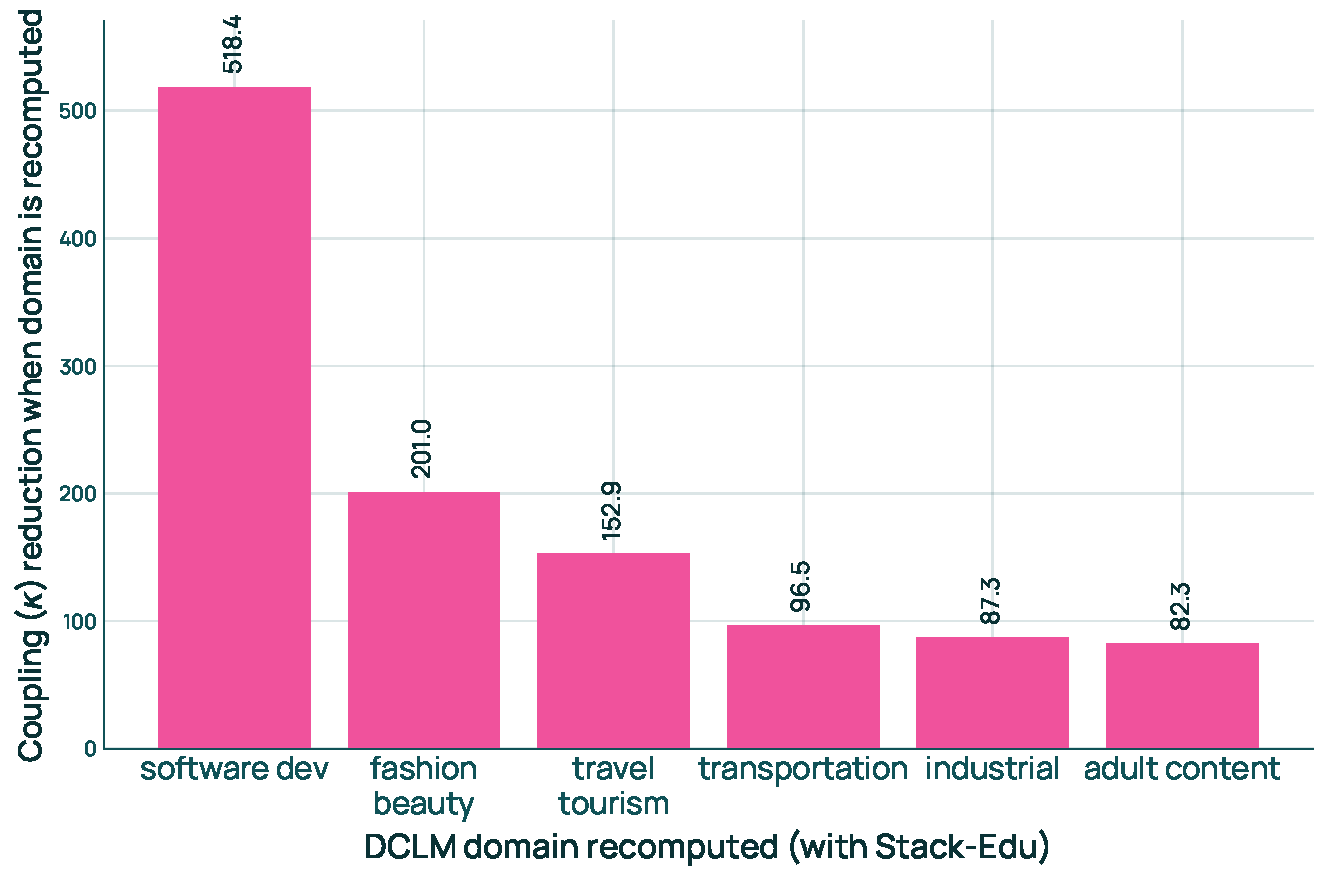
\includegraphics[width=0.6\linewidth]{figs/contribution_2/theorem2_validation_kappa_reduction.pdf}
    \caption{The top-6 DCLM domains for which recomputation results in the greatest reduction in $\kappa$ for $\D$=DCLM, $\D'$=DCLM+Stack-Edu. The reduction from recomputing DCLM:software development via \partialmixreuse is substantially higher than recomputing other DCLM topics.}
    \label{fig:theorem2_validation_kappa_reduction}
\end{figure}